\section{Problema 2}

\subsection{Introducción}

En este problema se debe determinar el área total de un campo que queda protegida de una plaga de langostas. Para considerar aislada una porción del mismo, ésta debe estar completamente encerrada por vallas de altura mayor o igual a la del salto de las langostas. A partir de entender esto, pensamos de qué manera podíamos modelar el campo, partirlo en "porciones" (que luego llamaríamos \textit{parcelas}), y recorrerlas chequeando si podíamos infestarlas de langostas. Realizando este recorrido, esperábamos lograr identificar el área infestada y contando con el área total, obtener mediante una simple resta el área protegida.\\
\indent Debido a cómo está presentado el problema, y los datos de entrada, consideramos el campo como el primer cuadrante de un sistema de ejes cartesianos. Así, el molino donde se ubica la Tía queda representado por el origen - $(0,0)$ - y cada valla se ubica en el plano con respecto a este punto. Además, a partir de la longitud y orientiacón de cada valla inferimos el extremo donde termina. De esta manera, al procesarlas todas, pudimos obtener cuáles eran las coordenadas máximas en sentido del eje de ordenadas y abscisas, con lo cual fijamos los límites del campo sumando uno a esos valores.\\
\indent En un primer momento nos propusimos modelar el campo utilizando esta información pero volcándola en una matriz donde cada posición de la misma se correspondiera con un sector del campo de lado $1x1$. Nuestra idea era posicionar las vallas en la matriz, determinando qué cuadrados quedaban bloqueados, y luego infestar de alguna manera pintando las posiciones de la matriz a las que sí podíamos acceder. Rápidamente desistimos de esta idea (a pesar de que luego la retomaríamos optimizando nuestras estructuras) dado que manejarnos con esa matriz no nos permitía cumplir con la cota de complejidad pedida. Las dimensiones de la matriz hubieran sido proporcionales a la superficie del campo, la cual a su vez quedaba determinada por la ubicación de una valla, variable sobre la cual no podíamos suponer nada y no se relacionaba con las magnitudes que necesitábamos contar.\\
\indent El segundo intento consistió en pensar cada valla como un nodo de un grafo, donde las aristas estuvieran representadas por las intersecciones entre las vallas. Luego, los vecinos de un nodo/valla serían otros nodos/vallas con los que se tocara en cualquier punto. Viéndolo así, buscamos interpretar las porciones completamente valladas como los ciclos de ese grafo. Una vez que tuvieramos identificados los ciclos, debíamos ver cuáles eran válidos, cuáles incluían a otros, y así procesar demasiados casos particulares. No pudimos llegar a esa instancia, pues antes nos encontramos con la dificultad de contar e identificar ciclos. Sin embargo, al pensar en cómo podíamos clasificar los ciclos, introdujimos un detalle que luego perduraría en nuestra solución final: a medida que procesamos cada valla para alojarla en nuestra estructura dejamos de lado aquella cuya altura sea menor a la que saltan las langostas. Así nos aseguramos que en el resto del problema vamos a mirar vallas que sean candidatas a proteger una porción del campo, con lo cual prescindimos de realizar este chequeo y mirar vallas innecesariamente.\\
\indent Frente a un panorama incierto, y habiendo descartado dos intentos de solución, logramos desarrollar una tercera idea que terminaría siendo correcta para la resolución del problema tanto en términos de la solución esperada como de la complejidad temporal. 

\subsection{Representación del Problema}

El primer boceto de solución con que contamos intentaba trazar una cuadrícula sobre el campo y luego implementar eso sobre una matriz. Esto nos obligaba a movernos de a un paso a medida que infestabamos el terreno, transformando nuestra complejidad en algo que no se relacionaba con la cantidad de vallas, y que seguramente fuera muy superior a este número. Ahora bien, considerando este movimiento, concebimos que no tenía sentido pensar que la plaga de langostas se moviera en una dirección dada de a pasos tan pequeños ya que en última instancia podría moverse hasta que se topara con una valla, infestando en un solo paso grande varios de nuestros pequeños sectores anteriores.\\
\indent Dividimos entonces la representación del campo en distintas etapas de procesamiento (ver \textbf{Fig. ~\ref{fig:ej2Mapeo} }). Primero, extendimos las vallas iniciales en megavallas que atravesaran el terreno del campo de un extremo a otro. Para esto contamos con dos diccionarios de megavallas, uno correspondiente a las verticales y otro a las horizontales. Cada definición se hace en base a una clave (entero) que representa la coordenada vertical u horizontal en que se extiende esa megavalla, y un significado que no es otra cosa que una lista de las vallas originales que viven en ese segmento y cuya altura impide el salto de las langostas. Además, la manera en que representamos las vallas es a través de un par de coordenadas, cuyas componentes $x$ e $y$ indican el comienzo y fin de la valla respectivamente.

\clearpage

\begin{figure}[h]
\centering                                                       
        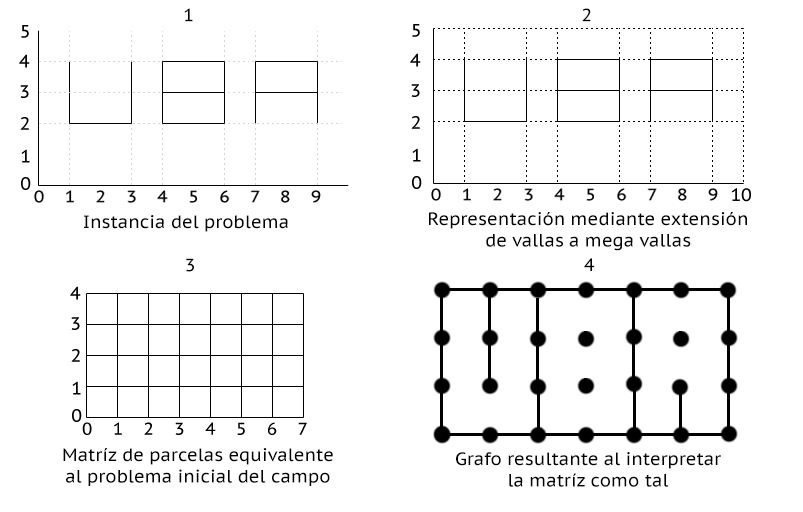
\includegraphics[width=320pt]{./figs/mapeoParcelas.png}
	\caption{Transformación del Problema Inicial}
	\label{fig:ej2Mapeo}
\end{figure}

Como se puede observar en la segunda imagen de la Fig. anterior, las intersecciones de las megavallas definen una cuadrícula de parcelas cuyo tamaño es variable y heterogéneo. Sin embargo, todas tienen forma rectangular, y a partir de la información almacenada hasta el momento es posible determinar su área y si el acceso a las parcelas contiguas está impedido o no por algún tramo de valla. Esto nos permitió armar una matriz que representara esta cuadrícula, de dimensiones $\#megavallasHor*\#megavallasVer$, y cuyas posiciones alojaran un objeto de tipo $Parcela$ que contuviera la información antes mencionada, además de agregar un atributo booleano para determinar si la parcela era infestable (necesario para recorrer la matriz con una adaptación de `BFS'). Este procesamiento se realiza a través de la función $armarParcelas$ (ver \textsl{Pseudocódigo 2}). Para lograr el correcto armado y mapeo del campo a esta matriz necesitamos contar con las megavallas ordenadas en forma ascendente (garantizado por el diccionario) así como también las vallas contenidas en cada una. En un principio, implementamos cada megavalla como otro diccionario que tuviera como clave el comienzo de una valla y como significado su fin. Esto nos garantizaba el orden necesario para recorrerlas, pero nos imponía un costo logarítmico para acceder a su significado. Dado que esto nos arruinaba la complejidad, acudimos a la implementación de la colección de vallas mediante una lista de manera tal que, al terminar de procesar todas las vallas, ordenáramos cada colección y así pudieramos acceder a toda su información en tiempo constante. Por eso, en la resolución del problema, hay un llamado al método de Campo $ordenarVallas$ antes de armar la matriz de parcelas, pues en otro caso el algoritmo no sería correcto.\\
\indent Esta matriz de parcelas se corresponde con la etapa número 3 de la Figura ~\ref{fig:ej2Mapeo}. Como se explica en el análisis de complejidad, esta vez sí podemos pagar el costo de recorrer la matriz, ya que sus dimensiones se encuentran en función de la magnitud que nos interesa (\#vallas). Al interpretarla como un grafo, las posiciones (parcelas) pasaron a ser los nodos, mientras que la arista entre un par de nodos implica que las langostas pueden moverse de entre ambas parcelas contiguas (ver Fig. ~\ref{fig:ej2Mapeo}.4). Luego, todo el área que pudiera ser infestada por estos desalmados crustáceos representaría una componente conexa del grafo. Supusimos entonces que la plaga comenzaba a infestar el campo desde los bordes, con lo cual partiendo de la parcela origen aplicamos una adaptación de 'BFS' ($buscarArea$, \textsl{Pseudocódigo 3}) para infestar la componente conexa que contuviera los bordes. A través de este recorrido contamos el área que podía ser infestada, y luego se lo restamos al área total.

\clearpage


\subsection{Pseudocódigos}

\begin{algorithm}
\caption{buscarArea (\textbf{in/out} campo: \textsl{Campo}) $\rightarrow$ res: \textsl{Integer}}
\begin{algorithmic}[1]

\STATE $cola \leftarrow$ crear cola de parcelas vacía
\STATE marcar $parcela$ $origen$ del campo como infestable
\STATE agregar $parcela$ $origen$ a la cola
\STATE $areaInfestada \leftarrow 0$

\WHILE{hay parcelas en la $cola$}
	\STATE $parcela \leftarrow$ pop primer elemento de la cola
	\STATE $areaInfestada \leftarrow areaInfestada$ $+$ área de $parcela$ 
	\STATE agregar parcelas contiguas a $parcela$ que se puedan infestar
\ENDWHILE
\RETURN área de $campo$ - $areaInfestada$
\end{algorithmic}
\end{algorithm}

\begin{algorithm}
\caption{armarParcelas (\textbf{in/out} campo: \textsl{Campo})}
\begin{algorithmic}[1]

\STATE $cantH \leftarrow$ cantidad de megavallas horizontales en el $campo$
\STATE $cantV \leftarrow$ cantidad de megavallas verticales en el $campo$
\STATE $cuadricula \leftarrow$ armar matriz de $cantH*cantV$
\WHILE{hay megavallas horizontales}
	\WHILE{hay megavallas verticales}
		\STATE crear una $parcela$ dada por las megavallas que la encierran
		\STATE definir en $parcela$ si se puede infestar en cada dirección
		\STATE definir en $parcela$ el área que comprende
		\STATE asignar $parcela$ a la posición correspondiente en $cuadricula$
	\ENDWHILE
\ENDWHILE
\STATE guardar $cuadricula$ en $campo$
\end{algorithmic}
\end{algorithm}

\begin{algorithm}
\caption{entranLoBicho (\textbf{in/out} megavalla: \textsl{Megavalla}, \textbf{in/out} inicio, fin: \textsl{Integer}) $\rightarrow$ res: \textsl{boolean}}
\begin{algorithmic}[1]

\STATE $res \leftarrow true$
\WHILE{haya vallas en $megavalla$}
	\STATE tomamos una $valla$ de la lista
	\IF{extremo inicial de la valla $> inicio$}
		\STATE \textbf{fin}
	\ELSE
		\IF{inicio y fin se encuentran entre los extremos de la valla}
			\STATE res $\leftarrow false$
			\STATE \textbf{fin}
		\ELSE
			\STATE $inicio \leftarrow$ extremo final de $valla$
		\ENDIF
	\ENDIF
\ENDWHILE
\RETURN $res$
\end{algorithmic}
\end{algorithm}

\clearpage

\subsection{Demostración de Correctitud}

Para ver la correctitud del programa, es necesario analizar sus distintas etapas por separado y demostrar que cada una cumple con comportamiento descrito en el modelado del problema. La propuesta para esta demostración es comenzar desde el final y asumir que si valen ciertas condiciones sobre los parámetros de entrada, entonces el algoritmo $buscarArea$ resuelve el problema correctamente. Luego, basta con ir hacia atrás y probar que las distintas funciones que utilizamos para construir esos parámetros garantizan esas condiciones.\\

\textbf{Correctitud de \textit{buscarArea} }

\indent Para esta función contamos con un objeto de tipo $Campo$ que posee almacenada y procesada toda la información necesaria sobre la instancia del problema. En particular, nos interesa acceder a su matriz de parcelas y recorrerla tratando de infestar todo el terreno. Recordemos que cada parcela $p$ es rectangular y por lo tanto posee un entero indicando su área, una coordenada que hace referencia a su posición $(i,j)$ en la matriz, y cuatro booleanos que indican si por cada uno de sus cuatro lados se puede infestar la parcela contigua. Además, cuenta con un flag propio que indica si es infestable. Para el correcto funcionamiento de este algoritmo de búsqueda, todas las parcelas de la matriz deben tener este último booleano en $false$, pero sí deben contar con los indicadores correctos sobre si es posible infestar parcelas contiguas. Dado que esta función es una adaptación de `BFS', a partir de una parcela dada irá agregarando a una cola aquellas parcelas contiguas que puedan ser infestadas y ya no hayan sido marcadas como tales (el equivalente a haber visitado un nodo).\\
\indent Debido a cómo fue construída, tanto la primera y última fila de la matriz como su primera y última columna corresponden a bordes del campo cuyas parcelas son infestables, pues asumimos que la plaga proviene desde cualquier dirección hacia el campo. Como esto impacta sobre el área total del campo, en principio el borde puede determinarse de manera arbitraria: lo importante es que exista, ya que sino el algoritmo no funcionaría como esperamos.\\
\indent Sea entonces $mp$ la matriz de parcelas de dimensiones $\#megaVallasH*\#megaVallasV$, este algoritmo comienza accediendo a la posición $(0,0)$ de la matriz para tomar la parcela $p_{0}$ y asignarle la condición de `infestable'; luego la agrega a la cola y comienza el ciclo iterativo de recorrido. El invariante de nuestro algoritmo determina que cualquier parcela agregada a la cola puede ser infestada a través de alguna de sus parcelas vecinas (lo cual interpretamos como que exista una arista entre ambos nodos/parcelas), con lo cual esta suerte de `BFS' se irá moviendo por la componente conexa que incluya a $p_{0}$ y a través de un efecto dominó infestará todas las parcelas en esta componente. Dado que garantizamos que hubiera al menos una fila o columna de parcelas borde infestables en cada extremo alrededor de todo el campo, cualquier parcela que no esté contenida en la componente conexa mencionada habrá quedado a salvo de las langostas gracias a su vallado, y por ende al restar el área infestada por el algoritmo al área total del campo habremos obtenido el área protegida total que se buscaba.\\
\indent El ciclo de la función itera mientras la cola no esté vacía. Dado que la precondición antes de entrar por primera vez es que la cola posee a $p_{0}$ y esperamos que a partir de ésta se recorra toda la componente conexa que la incluye, el hecho de que la cola se vacíe en alguna iteración dada implica que se ha recorrido la componente en su totalidad, con lo cual el área infestada acumulada en la variable entera es correcta. Sólo resta ver que el desplazamiento a través de la matriz sea correcto.\\
\indent En una iteración del ciclo, se saca el primer elemento de la cola ($p_{k}$) y se acumula su área al área parcial infestada. Como se vio, toda parcela en la cola ya ha sido marcada como infestable. Sea $(i,j)$ la posición de $p_{i}$ en $mp$, se invoca a la auxiliar $infestarParcelasContiguas$ que chequea si $(i+1,j), (i,j+1), (i-1,j),(i,j-1) \in mp$. En los casos que esto se cumpla, esta función pregunta si la parcela $p_{l}$ contenida en cualquiera de esas posiciones ya ha sido infestada ($aka$ visitada) y si, en todo caso, puede ser infestada desde $(i,j)$ (o sea, existe una arista entre $p_{k}$ y $p_{l}$). En el caso en que ambas condiciones fueran verdaderas, se marca $p_{l}$ como infestada y se la agrega a la cola para luego tratar de infestar a sus parcelas contiguas. Todo esto muestra que nunca se visita una misma parcela dos veces, que se evalúan todas las parcelas que pasan por la cola y que, para cada una de ellas se chequea si se puede infestar en las cuatro direcciones posibles, demostrando que todo lo anterior cumple con lo esperado y que el comportamiento de esta función es correcto respecto de la solución pedida. \\

\textbf{Correctitud de \textit{armarParcelas} }

El correcto funcionamiento de $buscarArea$ se basa principalmente en la correcta representación de la matriz de parcelas. Esta función se encarga de tomar toda la información de la instancia almacenada en el objeto de tipo $Campo$ y transformarla en la matriz necesaria. En este momento de la ejecución del programa, contamos con todas las vallas correctamente cargadas en los diccionarios de megavallas horizontales y verticales respectivamente, y para cada megavalla su lista de vallas se encuentra ordenada de forma ascendente a partir del punto en que comienza cada una. La idea principal de esta función es iterar en orden ambos diccionarios y a partir de las intersecciones de estos segmentos generar las parcelas correspondientes, calculando su área y si pueden pasar langostas por sus lados. Veamos cómo funciona el armado:\\
\indent Al comienzo de la función se crea la matriz de parcelas vacía. Sus dimensiones corresponden a la cantidad de megavallas horizontales por la cantidad de verticales. El armado de la matriz se hace primero por filas, y por cada fila se recorren sus columnas. Esto se traslada a cómo se recorren las megavallas. Dado que estas son simplemente segmentos, necesitamos contar con dos de ellas para poder delimitar una franja. De esta manera, fijar una fila significa fijar dos iteradores sobre las megavallas horizontales distantes en una posición sobre el conjunto de claves. Luego, el segundo ciclo recorre las megavallas verticales moviendo de la misma manera dos iteradores defasados en una posición. Además, la función sincroniza un par de enteros $i,j$ con el movimiento de estos iteradores para mapear las parcelas resultantes a la matriz. En resumen, los iteradores proveen toda la información necesaria para delimitar cada parcela. Dos apuntan a las megavallas que delimitan sus lados Norte y Sur, y dos verticales a sus lados Este y Oeste. Sea $m_{i}$ una de estas vallas, y suponiendo que su dirección fuera horizontal, se la busca en el diccionario correspondiente y luego se le aplica el método $entranLoBicho$, pasándole como parámetros los enteros correspondientes a las megavallas verticales que la cortan (apuntados por los iteradores antes mencionados). Una vez que se repite este proceso para el resto de los lados, se asignan los correspondientes valores de verdad en el objeto Parcela, se la marca como no infestable, se almacena su área y se la asigna a la posición $(i,j)$ de la matriz.\\
\indent Finalmente, esta matriz se almacena en el objeto de tipo $Campo$, lista para ser recorrida por $buscarArea$.\\

\textbf{Correctitud de \textit{entranLoBicho}}

Esta es otra de las funciones cruciales en el correcto funcionamiento del programa. Dada una megavalla y dos puntos $x_{i}$, $x_{f}$ en esa dirección, determina si por el segmento que forman pueden pasar langostas. En otras palabras, busca a través de todas las vallas definidas en la megavalla si éstas logran cubrir la totalidad del segmento, lo cual implicaría que está vallado. Esto se realiza iterando a través de todas las vallas definidas, previamente ordenadas mediante el método $ordenarVallas$, y comparando sus extremos con los del segmento en cuestión. Al tomar una valla $v_{k}$ con extremos $v_{i}$ inicial y $v_{f}$ final, si $v_{i} > x_{i}$ entonces existe un hueco en el segmento y automáticamente termina la ejecución, devolviendo verdadero (pueden entrar los bichos). Caso contrario, se chequea si $x_{i} \leq v_{f}$. Si esto se cumple y además $x_{f} \leq v_{f}$, entonces todo el segmento está contenido en $v_{k}$ y se puede concluir que los bichos no pasarán. En caso de que la última condición no se cumpliera, se buscará si el segmento está protegido por las vallas restantes, por lo que se vuelve a iterar sobre las vallas utilizando el mismo procedimiento pero cambiando $x_{i}$ por $v_{f}$.


\clearpage

\subsection{Análisis de Complejidad}

\indent A continuación analizaremos la complejidad de cada una de las
estructuras que utilizamos para resolver el ejercicio. Una vez que hayamos
calculado cada una, podremos analizar la complejidad total del programa. Antes, algunas propiedades que utilizaremos:

\begin{flushleft}
\textbf{Lema 1:} ($\forall m \in$ megavallas) Sea $n$ la cantidad de vallas contenidas en $m$, se cumple: que $1 \leq n \leq \#vallasTotales$ (salvo las megavallas de los bordes que no contienen ninguna valla).\\

\textbf{Lema 2:} Sea $M$ la cantidad total de megavallas y dado que para que exista una megavalla debe contener al menos una valla, $M \leq \#vallasTotales$\\
\end{flushleft}

\begin{itemize}
\item \textbf{Clase Coordenada}\\
\indent Funciones que provee el módulo:
\begin{itemize}
 \item \textbf{Constructor}: Se asignan 2 enteros $\rightarrow$ $O(1)$ 
 \item \textbf{Comparator}: Dadas 2 coordenadas, compara cual es mayor mediante
comparaciones que toman tiempo contante $\rightarrow$ $O(1)$ 
\end{itemize}

\item \textbf{Clase Megavalla}\\
\indent Funciones que provee el módulo:
\begin{itemize}
 \item \textbf{Constructor}: Crea un $ArrayList$ vacío, operación que según la documentación
de $Java$ se realiza en tiempo constante $\rightarrow$ $O(1)$ 
 \item \textbf{insertar}: Crea una nueva coordenada (ya vimos que se realiza
en tiempo constante) y la agrega al $ArrayList$. Según la documentación de
$Java$ $\rightarrow$ $O(1)$ $amortizado$
 \item \textbf{entranLoBicho}: Dada una Megavalla y 2 enteros que representan posiciones en dicho elemento, se devuelve un booleano indicando si entre esas posiciones pueden pasar las langostas. El ciclo itera tantas veces como vallas haya en esa megavalla; en una vuelta del ciclo se accede a la valla mediante el iterador del $ArrayList$, lo cual es constante, así como también lo son las comparaciones entre enteros que se realizan. En el peor caso se ciclan todas las vallas que contiene dicha megavalla  $\rightarrow$ $O(vallasEnMegavalla)$
$\subset$ $O(vallas)$ 
\end{itemize}

\item \textbf{Clase Parcela}\\
\indent Funciones que provee el módulo:
\begin{itemize}
 \item \textbf{Constructor}: Crea una parcela nueva inicializando sus valores
con los que se pasan por parámetro. Cada Parcela posee 5 campos booleanos, una
Coordenada y un entero. Realizar estas 7 asignaciones toma tiempo
constante $\rightarrow$ $O(1)$ 
\end{itemize}

\item \textbf{Clase Campo}\\
\indent Funciones que provee el módulo:
\begin{itemize}
 \item \textbf{Constructor}: Recibe 2 diccionarios (implementados sobre $TreeMap$) y 2
enteros. Estas variables son asignadas a sus correspondientes campos en la
estructura. Como $Java$ pasa por referencia estos parámetros, estas
asignaciones se realizan en tiempo constante $\rightarrow$ $O(1)$ 

 \item \textbf{ordenarVallas}: Para cada clave en los diccionarios de megavallas horizontales y verticales, ordena
las vallas que forman parte de su significado a partir del campo $x$ de cada elemento Coordenada. Como
el significado de las megavallas es un $ArrayList$, se utiliza la función $sort$ de $Java$
(clase Collections) que ordena los elementos utilizando el algoritmo $MergeSort$ 
en tiempo $O(n$ $log(n))$, donde $n$ es la cantidad de elementos del arreglo. Llevado a nuestro caso:

\begin{itemize}
 \item \textbf{Verticales}: Sea $m$ la cantidad de megavallas verticales definidas en el diccionario, para cada megavalla $m_{i}$ notamos $n_{i}$  la cantidad de vallas presentes en el arreglo asociado a su significado. Por ende, ordenar cada uno de estos arreglos toma $O(n_i$ $log(n_i))$ que por el \textbf{Lema 1} $\subset O(vallas$ $log(vallas))$. Además, como $m \leq M$ (la cantidad de megavallas totales) usando el \textbf{Lema 2} se ve que $m \leq vallas$. Por lo tanto la complejidad total de este ciclo es $O(vallas^2$ $log(vallas))$

\item \textbf{Horizontales}: Al igual que en el caso de las vallas verticales, la complejidad de ordenarlas es $O(vallas^2$ $log(vallas))$
\end{itemize}

\indent Como los casos de vallas Verticales y Horizontales son disjuntos,
podemos decir que la complejidad de la función es $\rightarrow$ $O(vallas^2$
$log(vallas)$ $+$ $O(vallas^2$ $log(vallas)))$ $\subset$ $O(vallas^2$
$log(vallas))$ 
 
\clearpage
 
 \item \textbf{armarParcelas}: Para analizar esta función, nos referiremos al
Pseudocódigo presentado en la sección 2.3.	
 \begin{enumerate}
	\item Para obtener la cantidad de megavallas horizontales, pedimos el $keySet$ al diccionario en $O(1)$ y preguntamos su tamaño.
	\item Idem anterior. Además, por el \textbf{Lema 2}, ambas magnitudes tienen como cota superior a la cantidad total de vallas.
	\item Se arma una matriz de tamaño a lo sumo $vallas$ x $vallas$ $\rightarrow$ $O(vallas^2)$
  	\item El primer while cicla a lo sumo $vallas$ veces, y recorre las megavallas horizontales		
	\item El segundo recorre las megavallas verticales ($vallas$ veces también)
		\begin{IndentedEnumerate}
		\item Creamos una nueva parcela $\rightarrow$ $O(1)$
  		\item Calculamos $entranLoBicho$ para cada dirección (Norte, Sur, Este, Oeste) $\rightarrow$ $O(4*vallas)$ $\subset$ $O(vallas)$ 
  		\item Calculamos el área comprendida por las 4 megavallas $\rightarrow$ $O(1)$
  		\item Agregamos esta parcela a la matriz en tiempo constante, dado que la asignación de la parcela se hace por referencia $\rightarrow$ $O(1)$
	\end{IndentedEnumerate}		
 \end{enumerate}


\indent En total, por estar anidados ambos ciclos iteran en orden $O(vallas$ $*$ $vallas)$. En todas esas iteraciones se realizan operaciones constantes salvo los llamados a $entranLoBicho$ que cuestan $O(vallas)$.\\
 \indent Por lo tanto, podemos decir que la complejidad total de la función
es:\\ $O(vallas^2$ $+$ $vallas$ $*$ $vallas$ $*$ $vallas)$ $\subset$
$O(vallas^3)$

\end{itemize}

\item \textbf{Clase Ej2}\\
\indent Funciones que provee el módulo:
\begin{itemize}
 \item \textbf{infestarParcelasContiguas}: Dada una parcela $p$, un campo $c$ y
una cola de parcelas $cp$, se fija cual de las parcelas contiguas a $p$ en $c$
son infestables y las agrega a $cp$. \\
Para realizarlo, por cada dirección, comparamos números enteros, accedemos a una
posición de la matriz y le asignamos un booleano, agregamos una parcela a una
$LinkedList$, todas operaciones que se realizan en tiempo constante. Por lo
tanto la complejidad de la función es $\rightarrow$ $O(1)$
\item \textbf{buscarArea}: Como explicamos en la sección anterior, la idea de
esta función esta basada en un recorrido BFS. Veremos si tiene un
comportamiento similar en cuanto a la complejidad. Para analizarla, nos
referiremos al Pseudocódigo presentado en la sección 2.3.
\begin{enumerate}
 \item Creamos una nueva $LinkedList$ $\rightarrow$ $O(1)$
 \item Marcamos la parcela origen como infestable $\rightarrow$ $O(1)$
 \item Agregamos la parela origen a la cola $\rightarrow$ $O(1)$
 \item Asignamos un entero $\rightarrow$ $O(1)$
 \item Ciclamos mientras haya parcelas en la cola. Como vimos anteriormente, el
tamaño de la matriz esta acotado por $vallas^2$, por lo que en el peor caso (si todas las parcelas fueran infestables),
este ciclo va a ejecutarse $vallas^2$ veces.
\begin{IndentedEnumerate}
\item Sacamos el primer elemento de la cola $\rightarrow$ $O(1)$
\item Realizamos una cuenta entre enteros $\rightarrow$ $O(1)$
\item $O(infestarParcelasContiguas)$ $\rightarrow$ $O(1)$
\end{IndentedEnumerate}
\end{enumerate}

Realizamos operaciones en tiempo constante a lo sumo $vallas^2$ veces, por lo
que concluimos que la complejidad de la función es la del ciclo $\rightarrow O(vallas^2)$.

\item \textbf{resolverFile}: Dado un archivo de entrada resuelve el problema y
lo escribe en un archivo de salida. Esta función es la que nuclea a todas las
funciones descriptas anteriormente, por lo tanto, podemos decir que la
complejidad de esta función va a ser la complejidad final de nuestro programa.\\
\indent Como no debemos contar la complejidad de leer y escribir en los
archivos, analizaremos solo la complejidad del código a partir de que los datos
fueron levantados.\\
\indent Ciclamos por todas las vallas, levantando sus parámetros y fijándonos primero si su altura es suficiente para impedir el salto de las langostas. En caso afirmativo, la procesamos; si no, la desechamos y seguimos adelante.\\
Al procesar una valla, la clasificamos acorde a su orientación y luego chequeamos si alguno de sus extremos mejora el punto más distante en el campo (método mediante el cual estimamos su área). Estas operaciones se realizan en $O(1)$ dado que solo comparamos caracteres, enteros y asignamos estos últimos. Para agregarla a la estructura procedemos a ver en qué megavalla se inserta. Como los casos de vallas
horizontales y verticales son disjuntos, podemos analizar uno solo, dado que son iguales (pondremos a modo de ejemplo el caso vertical).\\
\indent Mediante la función $containsKey$ del diccionario podemos determinar si la megavalla que contiene a la valla en cuestión ya fue definida o no. Este chequeo toma tiempo logarítmico, es decir $O(log(megavallasVerticales))$ $\subset$ $O(log(vallas))$. A partir de su resultado, los dos casos posibles son:
\begin{itemize}
 \item \textbf{Ya existía la megavalla}: $get$ en el diccionario toma
$O(log(megavallasVerticales))$ $\subset$ $O(log(vallas))$ e insertar la valla en una
megavalla ($add$ $arrayList$) toma tiempo $O(1)$ amortizado. $\rightarrow$
$O(log(vallas))$
 \item \textbf{No existía la megavalla}: Crear una nueva megavalla se hace en
tiempo constante. Insertar la valla en la megavalla toma tiempo $O(1)$ amortizado. Insertar en el diccionario mediante la función $put$ toma tiempo $O(log(megavallasVerticales))$ $\subset$ $O(log(vallas))$  $\rightarrow$ $O(log(vallas))$
\end{itemize}

Por lo tanto podemos decir que la complejidad de armar los diccionarios de vallas horizontales y verticales es $O(vallas$ $log(vallas))$.\\
\indent Al finalizar el procesamiento de todas las vallas contamos con los puntos más lejanos en las direcciones vertical y horizontal. Luego sumando 1 a estos valores creamos las 4 megavallas de los bordes. Como ninguna de las 4 existía podemos tomar la complejidad que escribimos anteriormente $\rightarrow$ $O(4*log(vallas))$ $\subset$ $O(log(vallas))$\\

\indent Creamos un nuevo campo en $O(1)$ (por lo analizado en esa Clase)\\
\indent Ordenamos las vallas del campo en  $O(vallas^2$ $log(vallas))$.\\
\indent Armamos las parcelas de la matriz en $O(vallas^3)$.\\
\indent Por ultimo buscamos la cantidad de área a salvo mediante la función
buscarArea en $O(vallas^2)$.\\

\indent Por lo tanto, podemos decir que la \textbf{complejidad total} del programa es:\\
$O(vallas$ $log(vallas)$+$log(vallas)$+$vallas^2$ $log$ $vallas$+$vallas^3$+$vallas^2) \subset$ \textbf{$O(vallas^3)$}

\end{itemize}

\end{itemize}






